The coroutines library, the modularized standard library, and the executors have something in common: they are supposed to be part of C++23.


\subsubsubsection{8.1.1\hspace{0.2cm} The Coroutines Library}

Coroutines in C++20 are no more than a framework for the implementation of concrete coroutines. This means that it is up to the software developer to implement coroutines. The \href{https://github.com/lewissbaker/cppcoro}{cppcoro} library from Lewis Baker gives the first idea how a library of coroutines could look like. His library provides what C++20 could not offer: high-level coroutines.

\begin{tcolorbox}[colback=blue!5!white,colframe=blue!75!black,title={Distilled Information}]
The cppcoro library is based on the coroutines TS. The TS stands for technical specification and is the preliminary version of the coroutines functionality we get with C++20. Lewis will presumably port the cppcoro library from the coroutines TS to the coroutines defined in C++20. The library can be used on Windows (Visual Studio 2017) or Linux (Clang 5.0/6.0 and libc++). For my experiments, I used the following command line for all examples:

\hspace*{\fill} \\ %插入空行
\noindent
cppcoro command line
\begin{tcblisting}{commandshell={}}
clang++ -std=c++17 -fcoroutines-ts -Iinclude -stdlib=libc++ libcppcoro.a
  cppcoroTask.cpp -pthread
\end{tcblisting}

\begin{itemize}
\item 
-std=c++17: support for C++17

\item 
-fcoroutines-ts : support for the C++ coroutines TS

\item 
-Iinclude : cppcoro headers

\item 
-stdlib=libc++: \href{https://en.wikipedia.org/wiki/LLVM}{LLVM} implementation of the standard library

\item 
libcppcoro.a: cppcoro library
\end{itemize}

As I already mentioned, when cppcoro is based on C++20 coroutines, you can use them with each compiler that supports C++20. Additionally, they give you a flavor for the concrete coroutines we may get with C++23.

In the rest of this section to the coroutines library, I want to demonstrate a few examples that show the power of coroutines. My demonstration starts with the coroutine types.

\end{tcolorbox}

\hspace*{\fill} \\ %插入空行
\noindent
\textbf{8.1.1.1\hspace{0.2cm} Coroutine Types}

cppcoro has various kinds of tasks and generators.

\hspace*{\fill} \\ %插入空行
\noindent
\textbf{8.1.1.1.1\hspace{0.2cm} task<T>}

What is a task? This is the definition used in cppcoro:

\begin{itemize}
\item 
A task represents an asynchronous computation that is executed lazily in that the execution of the coroutine does not start until the task is awaited.
\end{itemize}

A task is a coroutine. In the following program, the function main waits for the function first, first waits for second, and second waits for third.

\hspace*{\fill} \\ %插入空行
\noindent
Coroutines first sleeping
\begin{lstlisting}[style=styleCXX]
// cppcoroTask.cpp

#include <chrono>
#include <iostream>
#include <string>
#include <thread>

#include <cppcoro/sync_wait.hpp>
#include <cppcoro/task.hpp>

using std::chrono::high_resolution_clock;
using std::chrono::time_point;
using std::chrono::duration;

using namespace std::chrono_literals;

auto getTimeSince(const time_point<high_resolution_clock>& start) {

	auto end = high_resolution_clock::now();
	duration<double> elapsed = end - start;
	return elapsed.count();

}

cppcoro::task<> third(const time_point<high_resolution_clock>& start) {
	
	std::this_thread::sleep_for(1s);
	std::cout << "Third waited " << getTimeSince(start) << " seconds." << '\n';
	
	co_return;

}

cppcoro::task<> second(const time_point<high_resolution_clock>& start) {

	auto thi = third(start);
	std::this_thread::sleep_for(1s);
	co_await thi;
	
	std::cout << "Second waited " << getTimeSince(start) << " seconds." << '\n';

}

cppcoro::task<> first(const time_point<high_resolution_clock>& start) {

	auto sec = second(start);
	std::this_thread::sleep_for(1s);
	co_await sec;
	
	std::cout << "First waited " << getTimeSince(start) << " seconds." << '\n';

}

int main() {

	std::cout << '\n';
	
	auto start = high_resolution_clock::now();
	cppcoro::sync_wait(first(start));
	
	std::cout << "Main waited " << getTimeSince(start) << " seconds." << '\n';
	
	std::cout << '\n';

}
\end{lstlisting}

Admittedly, the program doesn’t do anything meaningful, but it helps to understand the workflow of coroutines.

First of all, the main function can’t be a coroutine. cppcoro::sync\_wait (line 59) often serves, such as in this case, as a starting top-level task and waits until the task is finished. The coroutine first, similar to the other coroutines, gets as an argument the start time and displays its execution time. What does the coroutine first do? It starts the coroutine second (line 36 and 46), which is immediately paused, sleeps for a second, and resumes the coroutine via its handle sec (line 38 and 48). The coroutine second performs the same workflow, but not the coroutine third. As for third it is a coroutine that returns nothing and does not wait on another coroutine. When third is done, all other coroutines are executed. Consequently, each coroutine takes 3 seconds.

\begin{center}
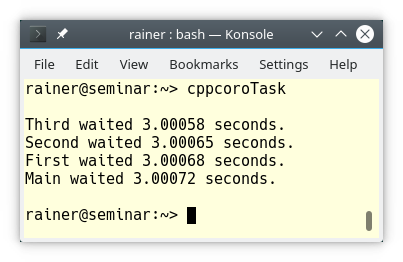
\includegraphics[width=0.8\textwidth]{content/5/chapter8/images/1.png}\\
Coroutines first sleeping
\end{center}

Let’s vary the program a little. What happens if the coroutines sleep after the co\_await call?

\hspace*{\fill} \\ %插入空行
\noindent
Coroutines first waiting
\begin{lstlisting}[style=styleCXX]
// cppcoroTask2.cpp

#include <chrono>
#include <iostream>
#include <string>
#include <thread>

#include <cppcoro/sync_wait.hpp>
#include <cppcoro/task.hpp>

using std::chrono::high_resolution_clock;
using std::chrono::time_point;
using std::chrono::duration;

using namespace std::chrono_literals;

auto getTimeSince(const time_point<::high_resolution_clock>& start) {

	auto end = high_resolution_clock::now();
	duration<double> elapsed = end - start;
	return elapsed.count();

}
cppcoro::task<> third(const time_point<high_resolution_clock>& start) {

	std::cout << "Third waited " << getTimeSince(start) << " seconds." << '\n';
	std::this_thread::sleep_for(1s);
	co_return;

}

cppcoro::task<> second(const time_point<high_resolution_clock>& start) {

	auto thi = third(start);
	co_await thi;
	
	std::cout << "Second waited " << getTimeSince(start) << " seconds." << '\n';
	std::this_thread::sleep_for(1s);

}

cppcoro::task<> first(const time_point<high_resolution_clock>& start) {

	auto sec = second(start);
	co_await sec;
	
	std::cout << "First waited " << getTimeSince(start) << " seconds." << '\n';
	std::this_thread::sleep_for(1s);

}

int main() {

	std::cout << '\n';
	
	auto start = ::high_resolution_clock::now();
	
	cppcoro::sync_wait(first(start));
	
	std::cout << "Main waited " << getTimeSince(start) << " seconds." << '\n';
	
	std::cout << '\n';

}
\end{lstlisting}

You may have guessed it. The main function waits 3 seconds, but each iteratively-invoked coroutine one second less.

The next coroutine that cppcoro provides is a generator<T>.

\hspace*{\fill} \\ %插入空行
\noindent
\textbf{8.1.1.1.2\hspace{0.2cm} generator<T>}

Here is cppcoro’s definition of a generator:

\begin{itemize}
\item 
A generator represents a coroutine type that produces a sequence of values of type T, where values are produced lazily and synchronously.
\end{itemize}

Without further ado, the program cppcoroGenerator.cpp demonstrates two generators in action.

\hspace*{\fill} \\ %插入空行
\noindent
Use of two generators
\begin{lstlisting}[style=styleCXX]
// cppcoroGenerator.cpp

#include <iostream>
#include <cppcoro/generator.hpp>

cppcoro::generator<char> hello() {
	co_yield 'h';
	co_yield 'e';
	co_yield 'l';
	co_yield 'l';
	co_yield 'o';
}

cppcoro::generator<const long long> fibonacci() {
	long long a = 0;
	long long b = 1;
	while (true) {
		co_yield b;
		auto tmp = a;
		a = b;
		b += tmp;
	}
}

int main() {

	std::cout << '\n';
	for (auto c: hello()) std::cout << c;
	
	std::cout << "\n\n";
	
	for (auto i: fibonacci()) {
		if (i > 1'000'000) break;
		std::cout << i << " ";
	}
	
	std::cout << "\n\n";

}
\end{lstlisting}

The first coroutine hello returns on request the next character and the coroutine fibonacci the next fibonacci number. fibonacci creates an infinite data stream. What happens in line 33? The range-based for loop triggers the execution of the coroutine. The first iteration starts the coroutines, returns the value at co\_yield b (line 18), and pauses. Subsequent calls of the range-based for loop resume the coroutine fibonacci and return the next fibonacci number.

\begin{center}
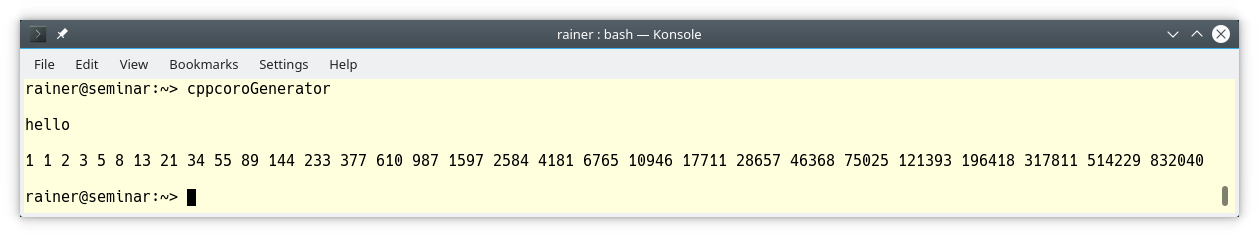
\includegraphics[width=0.8\textwidth]{content/5/chapter8/images/2.png}\\
Executing two generators
\end{center}

cppcoro provides more awaitable types.

\hspace*{\fill} \\ %插入空行
\noindent
\textbf{8.1.1.2\hspace{0.2cm} Awaitable Types}

cppcoro supports various awaitable types:

\subsubsubsection{8.1.2\hspace{0.2cm} Modularized Standard Library for Modules}

\subsubsubsection{8.1.3\hspace{0.2cm} Executors}

\subsubsubsection{8.1.4\hspace{0.2cm} The Network Library}


































